\section{Related Work}\label{sec:ch6:related} 
\subsection{Wavelets as a Front End}
Fujieda et.\ al.\ use a DWT in combination with a
CNN to do texture classification and image annotation 
\cite{fujieda_wavelet_2017, fujieda_wavelet_2018}. In particular, they take a
multiscale wavelet transform of the input image, combine the actviations at each
scale independently with learned weights, and feed these back into the network
where the activation resolution size matches the subband resolution. The
architecture block diagram is shown in \autoref{fig:ch6:fujieda}, taken from the
original paper.  This work found that their dubbed `Wavelet-CNN' could
outperform competetive non wavelet based CNNs on both texture classification and
image annotation.

\begin{figure}[bt]
  \centering
  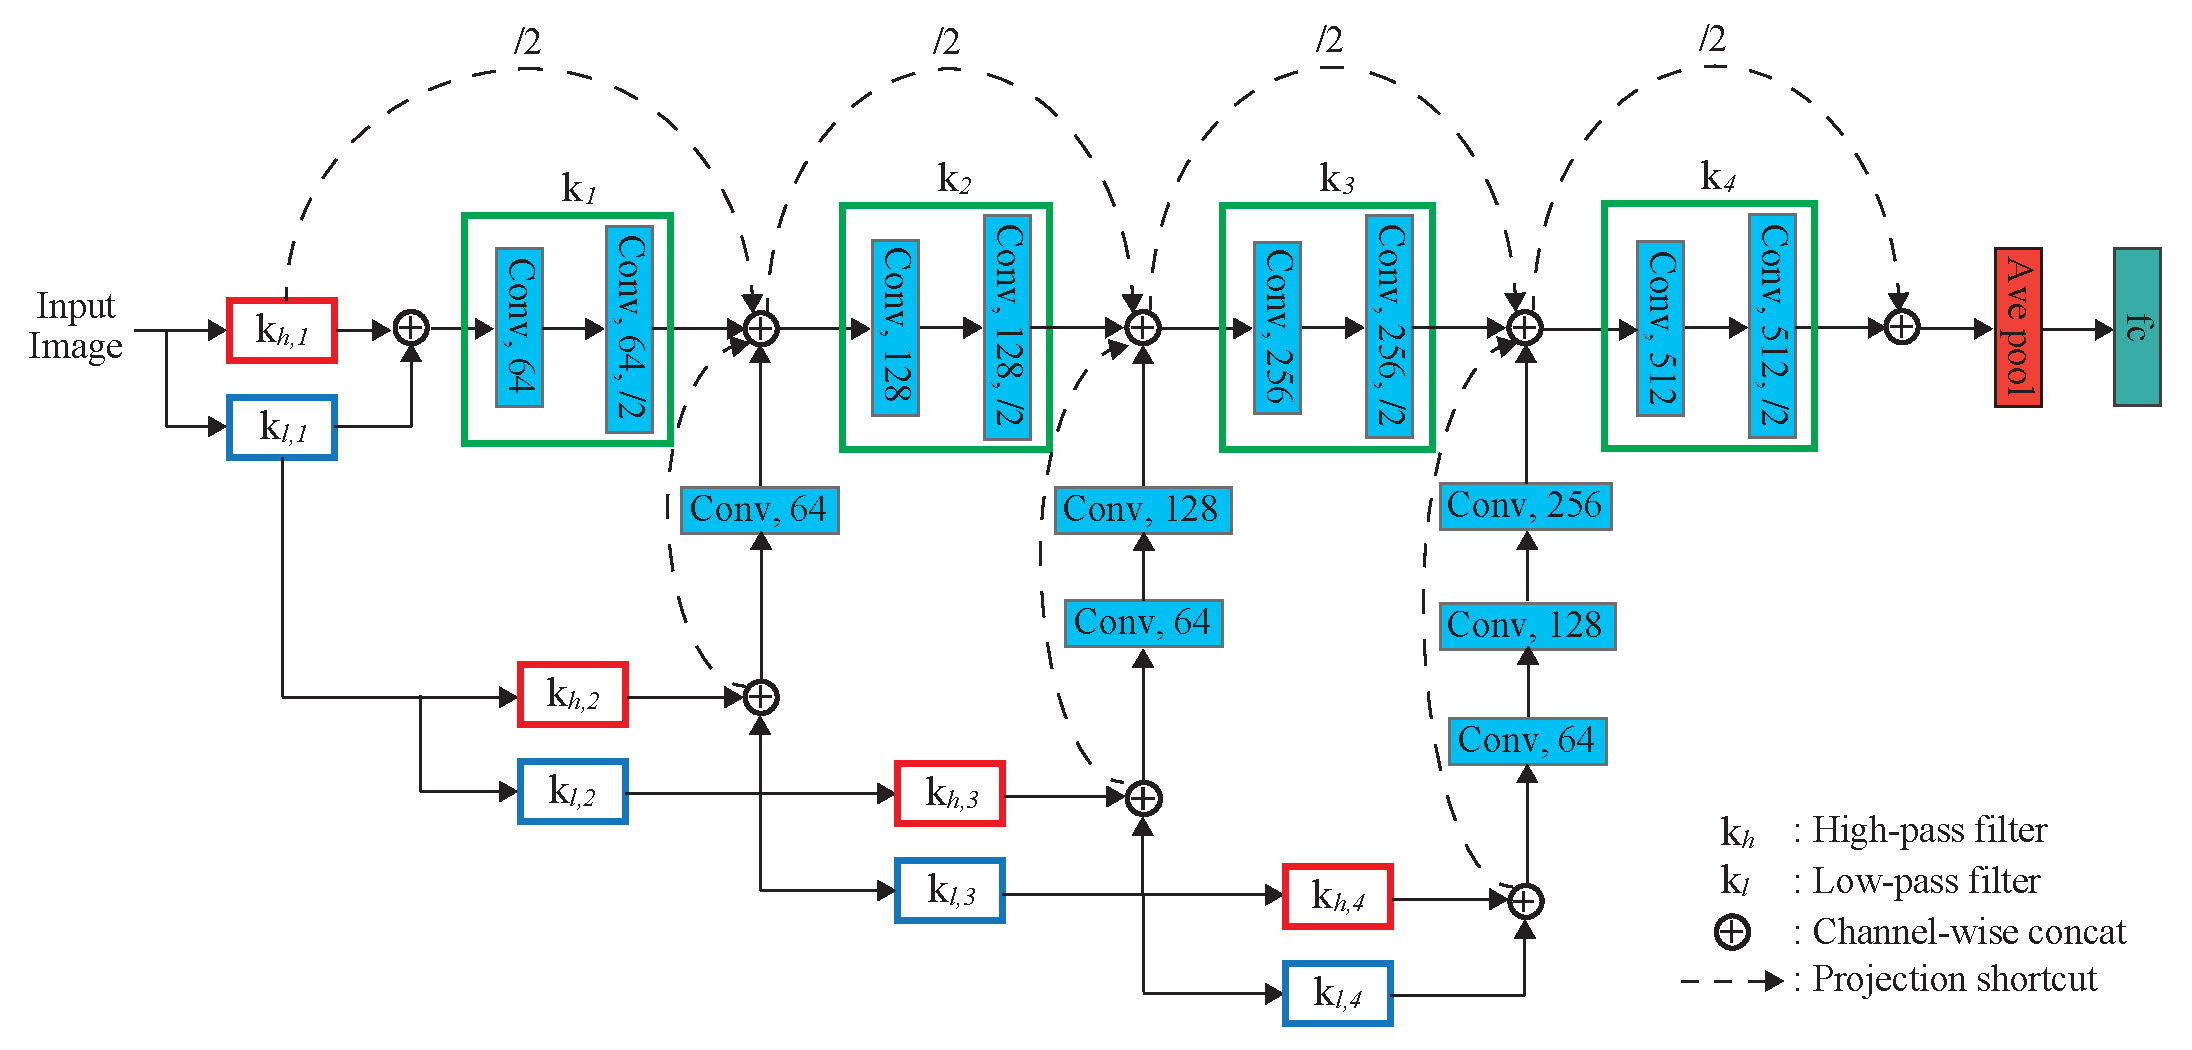
\includegraphics[width=\textwidth]{\imgpath/wavelet_CNN_3.pdf}
  \mycaption{Architecture using the DWT as a frontend to a CNN}{Figure 1 from
  \cite{fujieda_wavelet_2018}. Fujieda et.\ al.\ take a multiscale wavelet
  decomposition of the input before passing the input through a standard
  CNN\@. They learn convolutional layers independently on each subband and feed
  these back into the network at different depths, where the resolution of the
  subband and the network activations match.}
  \label{fig:ch6:fujieda}
\end{figure}

Several works also use wavelets in deep neural networks for super-resolution
\cite{guo_deep_2017} and for adding detail back into dense pixel-wise
segmentation tasks \cite{ma_detailed_2018}. These typically save wavelet
coefficients and use them for the reconstruction phase, so are a little less
applicable than the first work.

\subsection{Parameterizing filters in Fourier Domain}
In \citetitle{rippel_spectral_2015} \cite{rippel_spectral_2015}, Rippel et.\
al.\ explore parameterization of filters in the DFT domain.  Note that they do
not necessarily do the convolution in the Frequency
domain, they simply parameterize a filter $\vec{w} \in \reals[F\x C\x K\x K]$ as
a set of fourier coefficients $\hat{\vec{w}} \in \complexes[F\x C\x K \x \ceil{K/2}]$
(the reduced spatial size is a result of enforcing that the inverse DFT of their
filter to be real, so the parameterization is symmetric). On the forward pass of
the neural network, they take the inverse DFT of $\hat{\vec{w}}$ to obtain
$\vec{w}$ and then convolve this with the input $\vec{x}$ as a normal CNN
would do.\footnote{The convolution may be done by taking both the image and
filter back into the fourier space but this is typically decided by the
framework, which selects the optimal convolution strategy for the filter and
input size. Note that there is not necessarily a saving to be gained by
enforcing it to do convolution by product of FFTs, as the FFT size needed for
the filter will likely be larger than $K\x K$, which would require resampling
the coefficients}. 

\section{Introduction}

We would like to explore the possibility of using the wavelet domain as a
space to learn. Unlike the work of \cite{rippel_spectral_2015} which
only parameterized filters in the wavelet domain and transformed the filters
back to the pixel domain to do convolution, this chapter explores learning
wholly in the wavelet domain. I.e., we want to take a wavelet decomposition of
the input and learn gains to apply to these coefficients, and optionally return
to the pixel domain.

As neural network training involves presenting thousands of training samples on
memory limited GPUs, we want our layer to be fast and as memory efficient as
possible. To achieve this we would ideally choose to use a critically sampled
filter bank implementation.  The fast 2-D Discrete Wavelet Transform (DWT) is a
possible option, but it has two drawbacks: it has poor directional selectivity
and any alteration of wavelet coefficients will cause the aliasing cancelling
properties of the reconstructed signal to disappear. Another option is to use
the $\DTCWT$ \cite{selesnick_dual-tree_2005}. This comes with a memory overhead
which we discuss more in \autoref{sec:ch6:memory}, but it enables us to have
have better directional selectivity and allows for the possibility of returning
to the pixel domain with minimal aliasing \cite{kingsbury_complex_2001}.

We will look at the merits and drawbacks of both options, discuss how to
implement them, and finally run some experiments exploring how well these
layers work.

\subsection{Invertible Transforms and Optimization}
Note that an important point should be laboured about reparameterizing filters
in either the wavelet or Fourier domains. That is that any invertible linear
transform of the parameter space will not change the updates if a linear
optimization scheme (like standard gradient descent, or SGD with momentum) is
used. This is proved in \autoref{app:ch6:invertible}.
% Note that this is almost identical to a normal CNN, except it allows for
% slightly a reworked filter initialization and optimization. In fact, with linear optimizers
% such as SGD or momentum and using \ltwo regularization, this work is equivalent to
% do regular pixel domain convolution but applying is as well as 
% affecting optimizers that keep track of past updates (such as SGD with momentum, 
% Adam \cite{kingma_adam:_2014} or Adagrad). \autoref{fig:rippel_spectral_figs}
% shows the fourier and spatial representation of some of the filters in
% \cite{rippel_spectral_2015}, as well as histograms showing the sparsity of
% parameters and momenta for parameter updates. The lower mean in the distribution
% of parameter momenta indicates that fewer parameters are being updated in a
% constant direction.

% \subsubsection{Regularization}
% Due to Parseval's theorem, it is clear that applying an L2 regularization on the
% filter weights :

% $$\sum_i \lnorm{w_i}{2}^2 = \sum_i \lnorm{\hat{w}_i}{2}^2 = \sum_i
  % \lnorm{\real{\hat{w_i}}}{2}^2 + \lnorm{\imag{\hat{w_i}}}{2}^2 $$

% However can apply L1 regularization on the complex magnitude of the DFT filter
% weights to impose spectral sparsity.


% In fact it can easily be seen that any optimizer that uses linear combinations
% of gradients makes this new parameterization identical to parameterization in
% the spatial domain. Optimizers like Adam and Adagrad however have update rules
% that are not simply linear combinations of past gradients and so this affects
% the learning trajectory. For Adam, there is a step where the gradients are
% squared to estimate the variance of the parameter updates. 

% This shows that any work involving reparametrizing or rethinking filter
% convolution must be careful in what is done.

% Further to this, while the inspiration for the work comes from wanting to remain
% in the frequency domain, it is unsatisfying to simply parameterize filters there
% and then take the inverse DFT and perform normal convolution. Ideally we would
% like to fully take advantage of the benefits of a frequency representation.

% \begin{figure}
  % \centering
  % 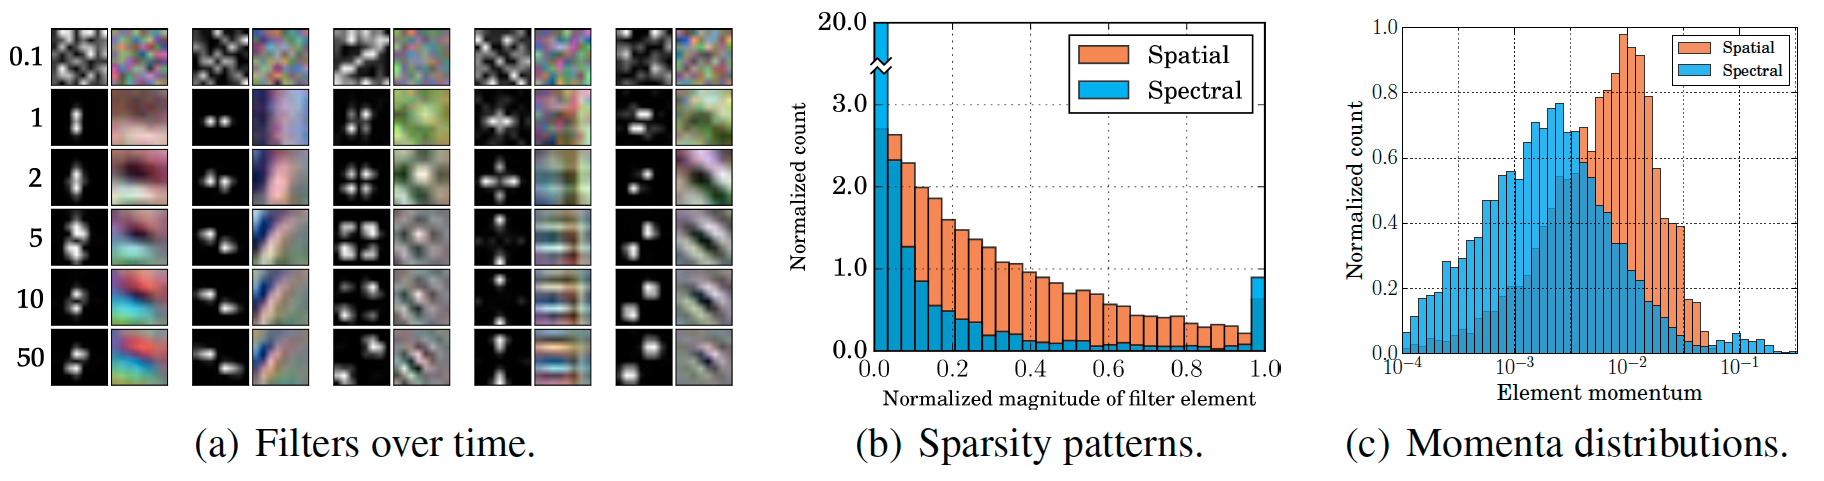
\includegraphics[width=\textwidth]{\imgpath/rippel.png}
  % \mycaption{Learning Dynamics of CNNs with DFT parameterization}{(a)
  % Progression over several epochs of filters parametrized in the frequency
  % domain. The left column shows the parameterized filter and the right column
  % its inverse DFT. (b) Sparsity patterns for different parameterizations -
  % spectral representations tend to be sparser. (c) Momenta distributions for
  % parameters of CNNs trained with and without spectral parameterization. In the
  % spectral parameterization fewer parameters are updated.  Image taken from
  % \cite{rippel_spectral_2015}.}
  % \label{fig:rippel_spectral_figs}
% \end{figure}


% \subsection{Spectral Pooling}
% The Spectral Pooling method introduced in \cite{rippel_spectral_2015} is
% described in the paper as:

% \begin{quote}
  % We assume we are given an input $\vec{x}\in \reals[M\x N]$, and some desired
  % output map dimensionality $H \x W$. First we compute the discrete Fourier
  % transform of the input into the frequency domain as $y = \mathcal{F}(\vec{x})
  % \in \complexes[M\x N]$, and assume that the DC componenet has been shifted to
  % the center of the domain as is standard practice. We then crop the frequency
  % representation by maintaining only the central $H\x W$ submatrix of
  % frequencies, which we denote as $\hat{\vec{y}} \in \complexes[H\x W]$. Finally, we
  % map this approximation back into the spatial domain by taking its inverse DFT
  % as $\hat{\vec{x}} = \mathcal{F}^{-1}(\hat{\vec{y}}) \in \reals[H\x W]$.
% \end{quote}

% While they have chosen to do this in the Fourier domain, this could also be
% achieved by convolving with a separable, resampled 2D sinc function of the
% appropriate frequencies for the horizontal and vertical directions:

% $$\hat{\vec{x}} = \frac{HW}{MN} \vec{x} \conv \F{sinc}(\frac{Hn_y}{M}) \conv
% \F{sinc}(\frac{Wn_x}{N})$$

% where $n_x \in \{??\}, n_y \in \{??\}$. Of course, sincs have infinite support
% in the time domain, so to achieve a similar result to spectral pooling you would
% have to convolve with windowed sincs, or do some other form of similar low pass
% filtering with resampling. In \cite{williams_wavelet_2018} they do exactly this
% and call it `wavelet pooling', which is just keeping the low-low output of a
% separable 2D DWT, or simply convolving with a separable lowpass filter. They
% experimentally showed that this was equivalent to spectral and average pooling.

% Note that speed ups could be achieved here if the convolution is done in the
% Fourier domain, as it would involve only computing the reduced spectrum size
% before taking inverse DFTs.


% \begin{enumerate}
  % \item the layers can easily replace standard convolutional layers if they
    % accept and return the same format;
  % \item we can learn both in the wavelet and pixel space.
% \end{enumerate}


